\documentclass{article}
\usepackage[utf8]{inputenc}
\usepackage{graphicx}
\usepackage{natbib}
\usepackage{chemfig}
\usepackage{siunitx}
\usepackage{amsmath}


\title{singlet fission}
\author{Anurag Singh }
\date{November 2019}

\begin{document}

Data of Napthalene monomer\\
Active space size = 8\\
Number of closed orbital =  30\\
Number of electron in active space = 8\\
\(S_{0}\) = -383.56099346\\
\(S_{1}\) = -383.38925996\\
\(T_{0}\) = -383.44193920\\
\(S_{1} - S_{0} \) = 0.1717335000000162 H ; 4.673108961900441 ev\\
\(T_{0} - S_{0} \) = 0.11905426000004127 H;  3.239633090565123 ev\\

Data of nap\_BN \\
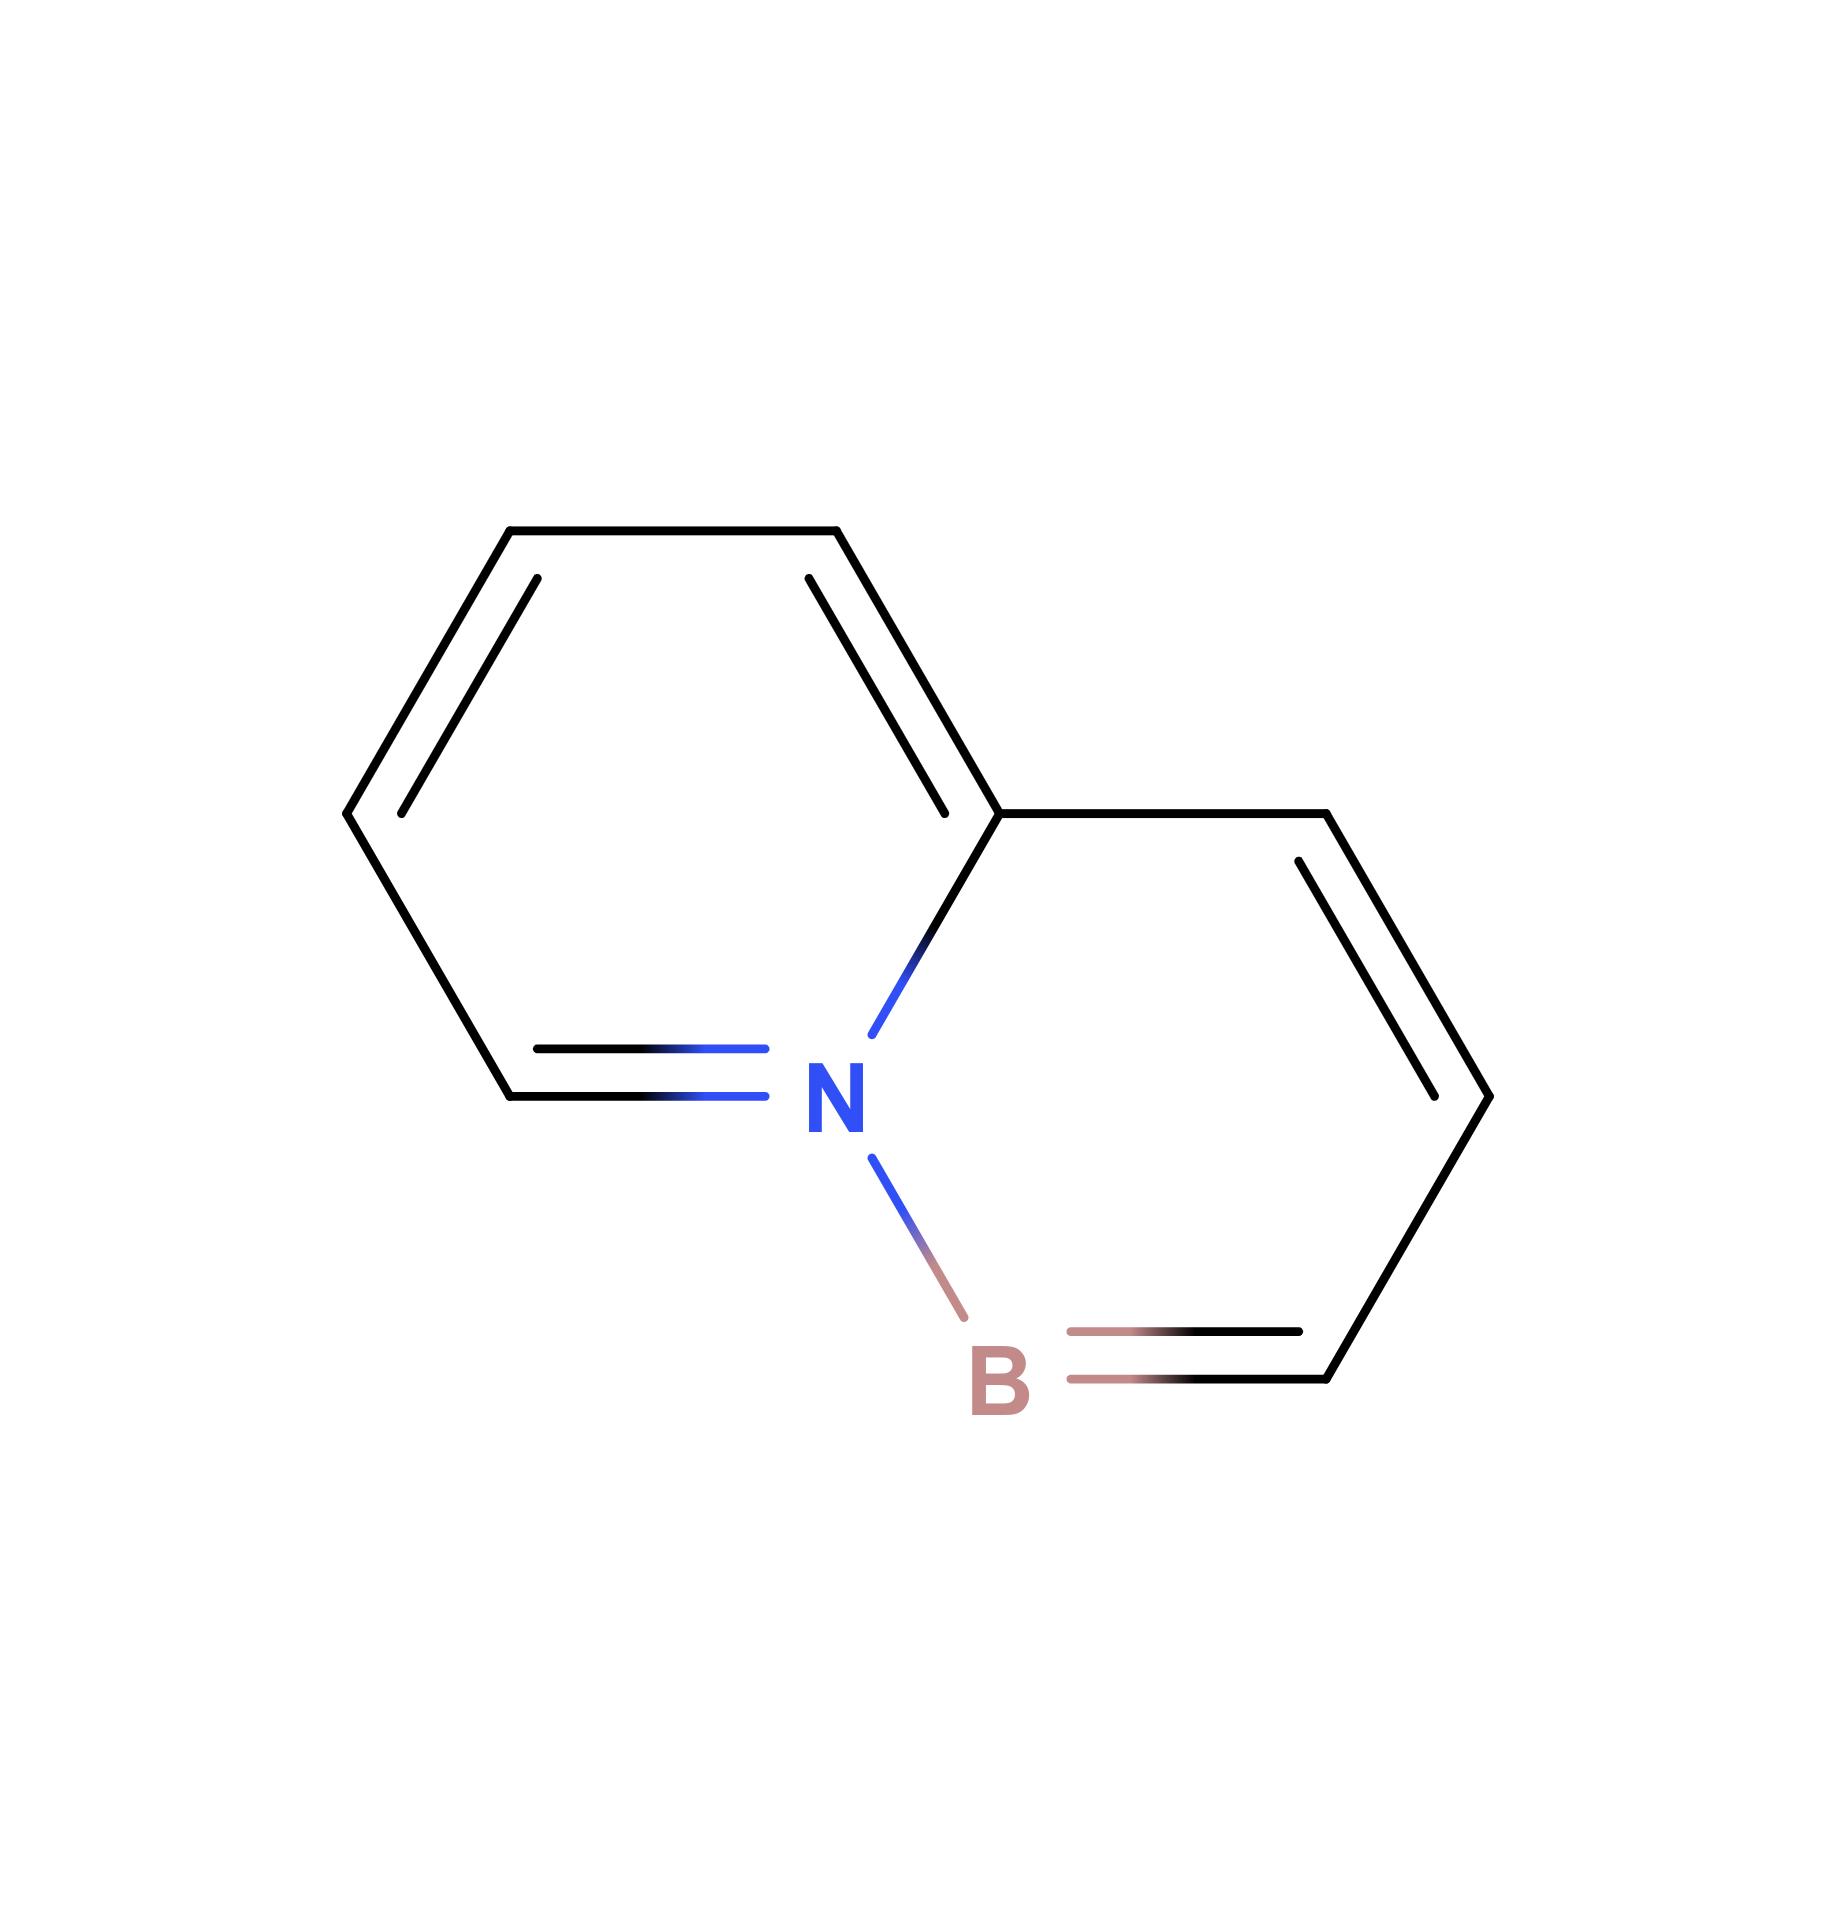
\includegraphics[scale=0.1]{Nap_BN.png}\\
Active space size = 8\\
Number of closed orbital = 30\\
Number of electron in active space = 8\\
\(S_{0}\) = -386.93035843\\
\(S_{1}\) = -386.79504438\\
\(T_{0}\) = -386.84171729\\
\(S_{1} - S_{0} \) = 0.1353140500000336 H ;  3.6820847401709145ev\\
\(T_{0} - S_{0} \) = 0.0886411399999929 H;  2.412049516995807 ev\\

Data For Napthalene dimer\\

The Dimer was created using Avogadro Its geometry was optimised using CAMB3LYP/cc-pVTZ the energy came out to be -770.775368021900 hartree. Then CASSCF calculation was performed on the resultant structure came out to be in accordance with publication By Oddershede et al. \cite{Oddershede_2004}\\*
\(S_{0}\) = -766.9980396 \\
\(S_{1}\)= -766.79708727 \\
\(T_{0}\) =  -766.86176967\\
\(S_{1} - S_{0}\) = 0.20095232999995005 H   ; p5.468194232560641 ev\\
\(T_{0} - S_{0} \) = 0.13626993000002585 H  ; 3.7080955732027037 ev\\
\begin{tabular}{c c c c}
\end{tabular}
\bibliographystyle{unsrt}

\bibliography{anurag}
\end{document}